\documentclass[10pt]{amsart}
%\documentclass[aps]{revtex4-2}
\usepackage[a4paper, margin=2cm]{geometry}

\usepackage{tikz}
\usetikzlibrary{quantikz}
\usepackage[utf8]{inputenc}
\usepackage{subcaption}
\usepackage{amsmath, amsfonts, hyperref,braket,amssymb}
% Define theorem-like environments with independent numbering
\newtheorem{theorem}{Theorem}
\newtheorem{lemma}{Lemma}
\newtheorem{conjecture}{Conjecture}
\newtheorem{definition}{Definition}
\newtheorem{example}{Example}
\newtheorem{proposition}{Proposition}
\newtheorem{corollary}{Corollary}
\newcommand{\A}{\mathcal{A}} 
\newcommand{\E}{\mathcal{E}}
\newcommand{\X}{\chi}

\newcommand{\dmat}[1]{{| #1 \rangle \langle #1 |}} 

\newcommand{\rl}[1]{{\rangle \langle}} 
\newcommand{\dm}[2]{\left|#1\right\rangle\left\langle#2\right|}

\newcommand{\EE}{{\mathcal E}}



\DeclareMathOperator{\Tr}{\textnormal{Tr}}


\title{Quantum algorithm for spectral sampling}
\author{Hobbes}
%\address{The Tiger}

\begin{document}
\maketitle

\begin{abstract}

    This note illustrates a method for sampling eigenstates of a class of Hermitian matrices on a quantum computer. The algorithm is presented in a framework utilising numerical integral transformations, to implement a spectral projection, that drives any state vector to a desired eigenspace, through a sequence of projectors parametrised by their schedules. 
    %, that drives any state to an state in the eigenspace within a given energy interval. 
    Numerical examples of the algorithm are given with illustrations.
    A proof-of-concept demonstration of the algorithm on IBMQ will be later done as an example. The asymptotic complexity of the algorithm is vaguely analysed and will be discussed as conjectures without any new results. The algorithmic method may be more generally formalised to engineer fine tuned dissipation schedules to do arbitrary BQP computations.
\end{abstract}


\section{Introduction}


We shall study quantum algorithms for sampling micro-canonical ensembles, i.e., pure states whose support is within a given energy interval. Given as input a classical description of $k$-local Hamiltonian $H_s = \sum_j h_j$ on $n$ qubits, energy interval $\Lambda_0, \Lambda_1 \in \mathbb{Q}$, such that $\Lambda_1-\Lambda_0 \in O(\frac{1}{poly(n)})$, and precision $\epsilon>0$, sample quantum states with almost full support on the span of the eigenstates with energy between $\Lambda_0, \Lambda_1$. Assume all inputs are given with $poly(n)$ bit rational approximation. 

Using quantum phase estimation this can then be extended to sample eigenstates between desired spectral intervals, when certain conditions of finite approximation of eigenvalues are met. 


\section{Notations}
Fix $H_s \equiv \sum_{j} \lambda_j \dmat{\phi_j}$ is a k-local  bounded norm Hamiltonian, acting on $n$ system qubits; denote energy interval $\Lambda = [\Lambda_0, \Lambda_1]$; and fix $\epsilon>0$.
Let $X \cong \sum_{j,k} x_{j,k} \dm{\phi_j}{\phi_k}$ be an efficiently implementable operation.  


\section{Algorithmic Setup}
The spectral sieve algorithm is an iterative algorithm that projects any initial state $\rho_0 = \sum_{jk} p_{i,j} | \phi_j \rangle \langle \phi_k |$ into the subspace $\chi_{[\Lambda_0, \Lambda_1]} = span(\{ \dmat{\phi_j} \}_{\lambda_j \in [\Lambda_0, \Lambda_1]})$, through a sequence of schedules. 

Define the map 
\begin{equation}
    \label{eq_map}
     \mathcal{E}_{X} : \rho_t \rightarrow Tr_A [ e^{iHt} (\dmat{0}^{m}_A\otimes \rho_t) e^{-iHt} ] 
     \end{equation}

where the Hamiltonian $H$ acts on $m$ ancillary qubits and $n$ system qubits, and defined as 
\begin{equation}
    \label{eq_H}
    H = I_{2^m} \otimes H_s + \sum_{j=1}^m a^{\dagger}_j \otimes \chi(X_j) + a_j \otimes \chi(X_j)^{\dagger}
\end{equation}
\textcolor{orange}{Numerically tested Oli idea- Use}
\begin{equation}
    \label{eq_OliH}
    H = \sum_{j=1}^m a^{\dagger}_j \otimes \chi(X_j) + a_j \otimes \chi(X_j)^{\dagger}
\end{equation}


where $\chi(X_j)$ is an approximation to the transformation of $X_j$ as,
\begin{equation}
    \label{eq_chi}
    \chi (X) = \int_R e^{itH_s} X f(t)dt \approx \sum_{j,k=1}^{N} \hat{f}({\lambda_j})x_{j,k} \dm{\phi_j}{\phi_k}
\end{equation}

with $f(t) \propto \frac{e^{-i \Lambda_0 t} - e^{-i \Lambda_1 t} }{it}$, such that 
$\hat{f}(\lambda_j) =  \begin{cases} 1, & \text{if } \lambda_j \in [\Lambda_0, \Lambda_1] \\ 0, & \text{otherwise } \end{cases}$,

\begin{proposition}
There exists an efficient implementation of the map $\EE_X$, as \eqref{eq_map}, whenever $\Lambda_1-\Lambda_0 \leq \frac{1}{poly(n)}$
\end{proposition}
\begin{proof}
    This will be shown using a combination of techniques and results on fast convergence of Newton-Cotes with Gauss Hermite Quadrature Rules, BCH expansion, and elementary matrix factorisation methods.

    Basic Idea: A quantum circuit for $U = e^{-iH}$

Recall a quadrature method to numerically integrate the real function $h$ as $I = \int_R h(t) dt$, using an approximation $I_{\epsilon}^{(L)} = \sum_{l=1}^L w_l h(t_l)$, where $w_l$ real valued called weights, and $\{t_1 \ldots t_L\}$ a set of real valued numbers called sample points. 
Specialising to our case, we use will use the same weights and sample points as  
Gaussian-Hermite quadrature. Observing that the function $|f(t)| \sim 1/t$ for large $t$ and exponential convergence of Gauss-Hermite, it suffices to $L$ growing polynomially in $n$, to be able to approximate the $\chi(X)$ up to exponential precision in max norm.

Thus \ref{eq_H} can be written as

\begin{align}
\label{eq_Hexpansion}
    H = & \sum_{j=1}^m a^{\dagger}_j \otimes \chi(X_j) + a_j \otimes \chi(X_j)^{\dagger} = \sum_{j=1}^m a^{\dagger}_j \otimes \big(\sum_{l=1}^L e^{iH_S t_l}X_jf(t_l) \big) + a_j \otimes \big(\sum_{l=1}^L X_je^{-iH_S t_l}\bar{f}(t_l) \big)  \\
     = & \sum_{j=1}^m \sum_{l=1}^L f(t_l)a^{\dagger}_j\otimes U_S(t_l)X + \bar{f}(t_l)a^{\dagger}_j\otimes X_j^{\dagger}U_S(-t_l)
\end{align}

Consider a vanishingly small norm approximation of $H = \sum_{j,l} H_\Delta$ with
$$H_{\Delta} = f(t_l)a^{\dagger}_j\otimes U_H(t_l)X + \bar{f}(t_l)a^{\dagger}_j\otimes X_j^{\dagger}U_H(-t_l)$$, and write it simply as $$H_{\Delta} = f(\tau)a^{\dagger}_j\otimes U_HX + \bar{f}(\tau)a^{\dagger}_j\otimes X^{\dagger} U_H^{\dagger} = \begin{bmatrix}
0 & f(\tau) U_H X \\
\bar{f}{\tau} X^{\dagger}U_H^{\dagger} & 0
\end{bmatrix}$$

The quantum circuit, $U_{\Delta} = e^{iH_\Delta}$ can be realised by observing 

\begin{align}
    exp(i H_\Delta) = & exp\big( i \begin{bmatrix}
0 & f(\tau) U_H X \\
\bar{f}{\tau} X^{\dagger}U_H^{\dagger} & 0
\end{bmatrix}  \big)    \\
=  & exp\big(i 
\begin{bmatrix}
U_H & 0 \\
0 & I 
\end{bmatrix} \cdot
\begin{bmatrix}
0 & f(\tau) X \\
\bar{f}{\tau} X^{\dagger} & 0
\end{bmatrix} \cdot
\begin{bmatrix} 
U_H^{\dagger} & 0 \\
0 & I 
\end{bmatrix} 
\\
= &  
\begin{bmatrix}
U_H & 0 \\
0 & I 
\end{bmatrix}  \cdot
exp\big(i \begin{bmatrix}
0 & f(\tau) X \\
\bar{f}{\tau} X^{\dagger} & 0
\end{bmatrix} \big) \cdot
\begin{bmatrix}
U_H^{\dagger} & 0 \\
0 & I 
\end{bmatrix} 
\end{align}

Simplify using $X = X^{\dagger}$, this is just a composition of a controlled $U_H$, followed by a phase-controlled $X$ then another controlled $U_H^{\dagger}$. In fact it is easy to even have $X$ to have same eigenvectors as a Haar random unitary $U_R$ (or k-design), by observing,

\begin{align}
    exp\big(i \begin{bmatrix}
0 & f(\tau) X \\
\bar{f}{\tau} X^{\dagger} & 0
\end{bmatrix} \big)  =  exp\big(i \begin{bmatrix}
0 & f(\tau) \\
\bar{f}{\tau} & 0
\end{bmatrix} \otimes X \big) = (I\otimes U_R ) exp\big(i \begin{bmatrix}
0 & f(\tau) \\
\bar{f}{\tau} & 0
\end{bmatrix} \otimes \sigma_x \big) (I\otimes U_R^{\dagger} )
\end{align}

Note that then $e^{iH_{\Delta}}$ admits an efficient circuit approximating it upto $\epsilon$ additive precision of size growing atmost polynomially in $n/\epsilon$. Subsequently the unitary $e^{iH}$ can be approximated upto $\varepsilon$ precision using a BCH-like formula as $e^{iH}= (e^{iH_{\Delta}})^{1/\Delta}$, since also $m$ and $L$ are atmost $poly(n)$ by definition and previously discussed quadrature arguments respectively. 
\end{proof}

\begin{figure}[h]
    \centering
\begin{quantikz}
%[transparent, row sep={0.8cm,between origins}]
\qw & \ctrl{0} & \qw & \gate[2,disable auto height]{f(t)} & \qw & \ctrl{0} & \qw\\
\qw & \gate[2,disable auto height]{U_H}\vqw{-1} & \gate[2,disable auto height]{U_R} & \qw & \gate[2,disable auto height]{U_R^{\dagger}} & \gate[2,disable auto height]{U_H^{\dagger}}\vqw{-1} & \qw\\
 \qw  &   \qw & \qw & \qwbundle{n-1} & \qw & \qw & \qw
\end{quantikz}
\caption{Schematic of a quantum circuit implementing $exp(iH_{\Delta})$}
    \label{fig:enter-label}
\end{figure}


\begin{conjecture}
Repeated applications of the map $\EE_X$ with a Haar random unitary $X$ on an initial on any state $\psi_0$ would converge to the state $\psi_T$, such that the spectrum of $\psi_T$ will be entirely supported on $\Lambda$
\end{conjecture}
\begin{proof}
    Let $P_0 = \sum_{i: \lambda_i \in [\Lambda_0, \Lambda_1]} \ket{\phi_i}\bra{\phi_i}$. Then 
    \begin{equation}
        \chi (X) \approx \sum_{j,k=1}^{N} \hat{f}({\lambda_j})x_{j,k} \dm{\phi_j}{\phi_k} = \sum_{j: \lambda_j \in [\Lambda_0, \Lambda_1]}\sum_{k=1}^{N} x_{j,k} \dm{\phi_j}{\phi_k} = P_0 X
    \end{equation}
    Therefore, \eqref{eq_H} can be written as:
    \begin{equation}
        H \approx  \sum_{j=1}^m a_j^{\dagger}\otimes P_0 X + a_j \otimes X^{\dagger} P_0
    \end{equation}
    Hence, we can express $e^{iHt}$ as:
    \begin{equation}
        e^{iHt} \approx \prod_j e^{i(a_j^{\dagger}\otimes P_0 X + a_j \otimes X^{\dagger} P_0)t}
    \end{equation}
    Define the following operators:
    \begin{align*}
        A &= \ket{1}\bra{0}_j \otimes P_0 X\\
        B &= \ket{0}\bra{1}_j \otimes X^{\dagger} P_0\\
        C &= \ket{1}\bra{1}_j\otimes P_0\\
        D &= \ket{0}\bra{0}_j\otimes X^{\dagger}P_0 X
    \end{align*}
    Then as $X$ is unitary and $P_0$ is a projector the following relations hold:
    \begin{align*}
        AB = C&, BA = D\\
        CC = C&, DD = D \\
        CA = A, DB = B&, AD = A, BC = B \\
        AA = 0, BB = 0,CB = 0, CD = 0&,DA= 0, DC = 0, AC = 0, BD = 0
    \end{align*}
    Hence, $(A+B)^2 = C+D$, $(C+D)^n = C+D$ and $(C+D)(A+B) = A+B$, so
    \begin{align}
    e^{i(A+B)t} &= \sum_{k=0}^{\infty} \frac{(it)^k}{k!} (A+B)^k \\
    &= \mathbb{I} + \sum_{k=1}^{\infty}\frac{(it)^{2k}}{(2k)!} (C+D) + \sum_{k=0}^{\infty}\frac{(it)^{2k+1}}{(2k+1)!} (A+B)\\
    &= \mathbb{I} + (\cos(t) -1) (C+D) + i\sin(t)(A+B)
    \end{align}
    By linearity we can consider the action of $\EE_X$ with a single ancillary qubit and then extend to $m$ ancillary qubits. With a single ancillary qubit the map is as follows:
    \begin{multline}
        \mathcal{E}_{X}(\rho) = Tr_A [ (\mathbb{I} + (\cos(t) -1) (C+D) + i\sin(t)(A+B)) \\(\dmat{0}_A\otimes \rho_t) (\mathbb{I} + (\cos(t) -1) (C+D) - i\sin(t)(A+B)) ] 
    \end{multline}
    \begin{equation}
        \mathcal{E}_{X}(\rho) = Tr_A [ (\dmat{0}_A\otimes\mathbb{I} + (\cos(t) -1) D + i\sin(t)A) \\(\dmat{0}_A\otimes \rho_t) (\dmat{0}_A\otimes\mathbb{I} + (\cos(t) -1) D - i\sin(t)B) ] 
    \end{equation}
    \begin{equation}
        \mathcal{E}_{X}(\rho) = (\mathbb{I} + (\cos(t) -1) X^{\dagger}P_0 X)\rho (\mathbb{I} + (\cos(t) -1) X^{\dagger}P_0 X) + \sin(t)^2P_0 X \rho X^{\dagger} P_0
    \end{equation}
    We wish to show that every application of this map never decreases the overlap with the desired energy eigenspace. Therefore, we need to demonstrate that $Tr(P_0 (\EE_x(\rho) -\rho)) \geq 0$.
    \begin{equation}
        Tr(P_0 (\EE_x(\rho) -\rho)) = Tr((\cos(t) -1) P_0X^{\dagger}P_0 X\rho +  (\cos(t) -1)P_0\rho X^{\dagger}P_0 X + (\cos(t) -1)^2 P_0X^{\dagger}P_0 X\rho X^{\dagger}P_0 X + \sin^2(t) P_0 X\rho X^{\dagger} P_0)
    \end{equation}
    Let $Q = X^{\dagger}P_0 X$, note that $Q^2 = Q$ ($Q$ is a projector), and remember that $Tr(PA) \leq Tr(A)$ if $P$ is a projector and $A$ is positive semi-definite:
    \begin{align}
        Tr(P_0 (\EE_x(\rho) -\rho)) &= Tr((\cos(t) -1) P_0Q\rho +  (\cos(t) -1)P_0\rho Q + (\cos(t) -1)^2 P_0Q\rho Q + \sin^2(t) Q\rho)\\
        &= Tr(2(\cos(t) -1) P_0Q\rho + (\cos(t) -1)^2 QP_0Q\rho + \sin^2(t) Q\rho)\\
        &\geq (2(\cos(t)-1) + (1-\cos t)^2 + \sin^2(t))Tr(  QP_0\rho ) =0
    \end{align}
    Therefore, applications of this map never decrease the overlap of the desired energy eigenspace. 
    
    Let us consider the application of this map to a single energy eigenstate $\ket{\phi_i}$. Let $\delta = \sum_{E_j \in \Lambda} |\bra{\phi_j}X\ket{\phi_i}|^2$. 
    \begin{equation}
        \mathcal{E}_{X}(\ket{\phi_i}\bra{\phi_i}) = (\mathbb{I} + (\cos(t) -1) X^{\dagger}P_0 X)\ket{\phi_i}\bra{\phi_i} (\mathbb{I} + (\cos(t) -1) X^{\dagger}P_0 X) + \sin(t)^2P_0 X \ket{\phi_i}\bra{\phi_i} X^{\dagger} P_0
    \end{equation}
    \begin{equation}
        \mathcal{E}_{X}(\ket{\phi_i}\bra{\phi_i}) = (\mathbb{I} + (\cos(t) -1) X^{\dagger}P_0 X)\ket{\phi_i}\bra{\phi_i} (\mathbb{I} + (\cos(t) -1) X^{\dagger}P_0 X) + \sin(t)^2 \delta^2 \ket{\lambda}\bra{\lambda}
    \end{equation}
    where $\ket{\lambda} = \sum_{E_j \in \Lambda} c_j \ket{\phi_j}$ for some $c_i$ such that $\sum_i |c_i|^2 = 1$. Therefore, a single application of $\EE_X$ to an energy eigenstate $\ket{\phi_i}$ such that $E_i \notin \Lambda$ produces a state with overlap $\delta^2 \sin^2(t)$ with $\Lambda$. As $X$ is a Haar random unitary on $D$ dimensions:
    \begin{equation}
        \mathbb{E}_X\mathbb{E}_\psi |\bra{\psi}X\ket{\psi}|^2 \sim \frac{1}{D}
    \end{equation}
    Let $Y_j$ be a unitary such that $Y_j\ket{\phi_i} = \ket{\phi_j}$. Then as $Y_j^{\dagger} X$ is also a Haar random unitary:
    \begin{equation}
\mathbb{E}_X |\bra{\psi_j}X\ket{\psi_i}|^2= \mathbb{E}_X |\bra{\psi_i}Y^{\dagger}_jX\ket{\psi_i}|^2 \sim \frac{1}{D}
    \end{equation}
    Therefore, $\mathbb{E}_X \delta = \frac{L}{D}$ where $L$ is the number of energy eigenstates in $\Lambda$. Therefore, if $L>0$ the expected overlap after a single application of our map to any energy eigenstate not in $\Lambda$ is greater than zero, and so as the overlap never decreases we have that our map converges to $\Lambda$ in finite time.
    % \begin{multline}
    %     \mathcal{E}_{X}(\ket{\phi_i}\bra{\phi_i})=\ket{\phi_i}\bra{\phi_i} +(\cos(t) -1) X^{\dagger}P_0 \ket{\phi_j}\bra{\phi_i} +  (\cos(t) -1)\ket{\phi_i}\bra{\phi_j} P_0 X +\\ (\cos(t) -1)^2 X^{\dagger}P_0 \ket{\phi_j}\bra{\phi_j} P_0 X + \sin^2(t) P_0 \ket{\phi_j}\bra{\phi_j}  P_0
    % \end{multline}
    % \begin{multline}
    %     \mathcal{E}_{X}(\ket{\phi_i}\bra{\phi_i})=\ket{\phi_i}\bra{\phi_i} +(\cos(t) -1) X^{\dagger} \ket{\phi_j}\bra{\phi_i} +  (\cos(t) -1)\ket{\phi_i}\bra{\phi_j} X +\\ (\cos(t) -1)^2 X^{\dagger} \ket{\phi_j}\bra{\phi_j}  X + \sin^2(t) \ket{\phi_j}\bra{\phi_j} 
    % \end{multline}
    % \begin{equation}
    %     \mathcal{E}_{X}(\ket{\phi_i}\bra{\phi_i})=\cos^2(t)\ket{\phi_i}\bra{\phi_i}  + \sin^2(t) \ket{\phi_j}\bra{\phi_j} 
    % \end{equation}
    
\end{proof}


\begin{conjecture}
Noisy conjecture
\end{conjecture}
\begin{proof}
    Define the following operators:
    \begin{align}
        A &= \ket{1}\bra{0}_j \otimes P X\\
        B &= \ket{1}\bra{1}_j\otimes P^2\\
        C &= \ket{0}\bra{0}_j\otimes X^{\dagger}P^2 X
    \end{align}
    Then as $X$ is unitary the following relations hold (assuming $P$ is hermitian):
    \begin{align*}
        AA^{\dagger} = B&, A^{\dagger} A = C\\
        AA = 0&, BC= 0 , CB = 0 
    \end{align*}
    Therefore, $(A+A^{\dagger})^2 = B+C$ and $(B+C)^k = B^k + C^k$, and hence:
    \begin{equation}
        (A+A^{\dagger})^{2k} = \ket{1}\bra{1}_j\otimes P^{2k} + \ket{0}\bra{0}_j\otimes X^{\dagger}P_0^{2k} X
    \end{equation}
    \begin{equation}
        (A+A^{\dagger})^{2k+1} = \ket{1}\bra{0}_j\otimes P^{2k+1}X + \ket{1}\bra{0}_j\otimes X^{\dagger}P_0^{2k+1}
    \end{equation}
    Therefore,
    \begin{multline}
        e^{i(A+A^{\dagger})} = \mathbb{I} + \sum_{k=1}^{\infty} \frac{(it)^{2k}}{(2k)!}(\ket{1}\bra{1}_j\otimes P^{2k} + \ket{0}\bra{0}_j\otimes X^{\dagger}P_0^{2k} X)+\\
        \sum_{k=0}^{\infty} \frac{(it)^{2k+1}}{(2k+1)!}(\ket{1}\bra{0}_j\otimes P^{2k+1}X + \ket{0}\bra{1}_j\otimes X^{\dagger}P_0^{2k+1})
    \end{multline}
    Let $P = P_0 + \epsilon \Gamma$ where $P_0$ is a projector and $\Gamma$ is a hermitian matrix, then:
    \begin{equation}
        P^k = (P_0 + \epsilon \Gamma)^k = P_0 + \epsilon(P_0 \Gamma + \Gamma P_0) + (k-2)\epsilon P_0 \Gamma P_0 + O(\epsilon^2)
    \end{equation}
    for $k\geq 2$. Let $R = P_0 \Gamma + \Gamma P_0$, then:
    \begin{multline}
        e^{i(A+A^{\dagger})} = \mathbb{I} + \sum_{k=1}^{\infty} \frac{(it)^{2k}}{(2k)!}(\ket{1}\bra{1}_j\otimes (P_0 + \epsilon R + (2k-2)\epsilon P_0 \Gamma P_0 + O(\epsilon^2)) +\\
        \ket{0}\bra{0}_j\otimes X^{\dagger}(P_0 + \epsilon R + (2k-2)\epsilon P_0 \Gamma P_0 + O(\epsilon^2)) X)+\\
        \sum_{k=1}^{\infty} \frac{(it)^{2k+1}}{(2k+1)!}(\ket{1}\bra{0}_j\otimes (P_0 + \epsilon R + (2k-1)\epsilon P_0 \Gamma P_0 + O(\epsilon^2))X + \ket{0}\bra{1}_j\otimes X^{\dagger}(P_0 + \epsilon R + (2k-1)\epsilon P_0 \Gamma P_0 + O(\epsilon^2))) \\
        +it(\ket{1}\bra{0}_j\otimes (P_0 + \epsilon\Gamma)X + \ket{0}\bra{1}_j\otimes X^{\dagger}(P_0 + \epsilon\Gamma))
    \end{multline}
    \begin{multline}
        e^{i(A+A^{\dagger})} = \mathbb{I} + (\cos(t)-1)(\ket{0}\bra{0}_j\otimes X^{\dagger}P_0 X + \ket{1}\bra{1}_j\otimes P_0) + i \sin(t) (\ket{1}\bra{0}_j \otimes P_0 X + \ket{0}\bra{1}_j \otimes X^{\dagger}P_0) + \\
        \epsilon(\cos(t)-1)(\ket{0}\bra{0}_j\otimes X^{\dagger}R X + \ket{1}\bra{1}_j\otimes R) + \\
        \epsilon(2 - 2 \cos(t) - t \sin(t))(\ket{0}\bra{0}_j\otimes X^{\dagger}P_0\Gamma P_0 X + \ket{1}\bra{1}_j\otimes P_0\Gamma P_0) + \\
        i\epsilon(\sin(t) -t)(\ket{1}\bra{0}_j \otimes R X + \ket{0}\bra{1}_j \otimes X^{\dagger}R) + \\
        i\epsilon (t + t \cos(t) - 2 \sin(t))(\ket{1}\bra{0}_j \otimes P_0\Gamma P_0 X + \ket{0}\bra{1}_j \otimes X^{\dagger}P_0\Gamma P_0) + \\
        i\epsilon t (\ket{1}\bra{0}_j \otimes \Gamma  X + \ket{0}\bra{1}_j \otimes X^{\dagger}\Gamma ) + O(\epsilon^2 t^2)
    \end{multline}
    \begin{multline}
        Tr[P_0(\mathbb{I} + (\cos(t) -1)Q + \epsilon(\cos (t) -1)(W + W^{\dagger}) + \epsilon(2 - 2\cos(t) - t\sin(t))M)\rho\\(\mathbb{I} + (\cos(t) -1)Q + \epsilon(\cos (t) -1)(W + W^{\dagger}) + \epsilon(2 - 2\cos(t) - t\sin(t))M) +\\ (sQ + \epsilon sW + \epsilon (t\cos(t) - \sin(t))M)\rho(sQ + \epsilon sW^{\dagger} + \epsilon (t\cos(t) - \sin(t))M) + O(\epsilon^2t^2)  - P_0\rho ]
    \end{multline}
        \begin{multline}
        Tr[(c-1)P_0 Q \rho + (c-1) QP_0 \rho + (c-1)^2 QP_0Q\rho + s^2 Q\rho +\\
        \epsilon( (c-1)(P_0 W + P_0 W^{\dagger} + W P_0 + W^{\dagger} P_0 + Q P_0 W + Q P_0 W^{\dagger} + WP_0 Q + W^{\dagger}P_0 Q) +\\ 
        (2 - 2c - ts)(P_0 M + M P_0 + M P_0 Q + Q P_0 M) + s^2 (W + W^{\dagger}) + 2(tc - s)s M) \rho + O(\epsilon^2t^2) ]
    \end{multline}
    \begin{multline}
        \geq Tr[QP_0(c-1)(  \rho - Q\rho) +\\
        \epsilon( (c-1)QP_0( 2W +  2W^{\dagger} + W P_0 + W^{\dagger} P_0 + WP_0 Q + W^{\dagger}P_0 Q) +\\ (2 - 2c - ts)QP_0( 2M + M P_0 + M P_0 Q) + s^2 W + (2tc - s)s M) \rho + O(\epsilon^2t^2) ]
    \end{multline}

\end{proof}

\section{Quantum Circuits}


\eqref{eq_H} can be written as:
    \begin{equation}
        \widetilde{H}^{\Lambda}_{\X} =  \sum_{j=1}^m \ket{1}\bra{0}_j \otimes P_{\Lambda}X + \ket{0}\bra{1}_j \otimes X^{\dagger} P_{\Lambda} = \begin{bmatrix}
            0 & X^{\dagger}P \\ PX & 0 
        \end{bmatrix} .
    \end{equation}

\begin{align}  
    A = exp(it \begin{bmatrix} 0 & X^{\dagger}P \\ PX & 0 \end{bmatrix} ) & = exp(it \begin{bmatrix} X^{\dagger} & 0 \\ 0 & I \end{bmatrix} \begin{bmatrix} 0 & P \\ P & 0 \end{bmatrix} \begin{bmatrix} X & 0 \\ 0 & I \end{bmatrix}) \\
    & = \begin{bmatrix} X^{\dagger} & 0 \\ 0 & I \end{bmatrix} exp(it \begin{bmatrix} 0 & P \\ P & 0 \end{bmatrix}) \begin{bmatrix} X & 0 \\ 0 & I \end{bmatrix} \\
    & = \begin{bmatrix} X^{\dagger} & 0 \\ 0 & I \end{bmatrix} exp( it \begin{bmatrix} 0 & \int_R U_t f(t)dt \\ (\int_R U_t f(t)dt)^{\dagger} & 0 \end{bmatrix}) \begin{bmatrix} X & 0 \\ 0 & I \end{bmatrix} \\
    & \approx \begin{bmatrix} X^{\dagger} & 0 \\ 0 & I \end{bmatrix} exp( it \begin{bmatrix} 0 & \sum_j U_j w_j \\ \sum_j U^{\dagger}_j w_j^* & 0 \end{bmatrix}) \begin{bmatrix} X & 0 \\ 0 & I \end{bmatrix} \\ 
    & = \begin{bmatrix} X^{\dagger} & 0 \\ 0 & I \end{bmatrix} \prod_j exp(it \begin{bmatrix} 0 &  U_j w_j \\  U^{\dagger}_j w_j^* & 0 \end{bmatrix}) \begin{bmatrix} X & 0 \\ 0 & I \end{bmatrix} \\
    & = \begin{bmatrix} X^{\dagger} & 0 \\ 0 & I \end{bmatrix} \prod_j exp(it \begin{bmatrix} 0 &  U_j w_j \\  U^{\dagger}_j w_j^* & 0 \end{bmatrix}) \begin{bmatrix} X & 0 \\ 0 & I \end{bmatrix} \\
    & = \begin{bmatrix} X^{\dagger} & 0 \\ 0 & I \end{bmatrix}
    (\prod_j 
    \begin{bmatrix} U_j^{\dagger} & 0 \\ 0 & I \end{bmatrix}
     exp(it \begin{bmatrix} w_j &  0 \\  0 & w_j^* \end{bmatrix})\begin{bmatrix} U & 0 \\ 0 & I \end{bmatrix} ) \begin{bmatrix} X & 0 \\ 0 & I \end{bmatrix} =: A^{(T)}
\end{align}

\begin{theorem}
$||A - A^(T)|| \leq O(\frac{1}{2^T})$
\end{theorem}
% \subsection{Thoughts}
% \textcolor{orange}{Note to Oli: To analyse the real implementation/error case, it suffices to extend this analysis to $\widetilde{P_0}X$, where $\widetilde{P_0} = P_0 + \varepsilon\Gamma$, where $\Gamma$ is a Gaussian random matrix with mean 0, and variance 1, and  $\varepsilon \sim \frac{1}{N^2}$. In our case, the approximation error will be really really small.}

% Let $V = V_G \oplus V_B$ be a vector space, and $\Pi_0, \Pi_1$ be projectors onto $V_G$ and $V_B$ respectively.

% For any state $\rho \in V$,
% $$ \rho = \Pi_0 \rho \Pi_0 + \Pi_1 \rho \Pi_0  + \Pi_0 \rho \Pi_1 +\Pi_1 \rho \Pi_1 \sim \begin{bmatrix}
%     \Pi_0 \rho \Pi_0  & \Pi_0 \rho \Pi_1 \\ 
%     \Pi_1 \rho \Pi_0  & \Pi_1 \rho \Pi_1 
% \end{bmatrix}$$

% $$\mathcal{E}(\rho) = Tr[\Pi_0 \mathcal{E}(\rho)]\cdot \Pi_0 \mathcal{E}(\rho) \Pi_0 + Tr[\Pi_1 \mathcal{E}(\rho)]\cdot \Pi_1 \mathcal{E}(\rho) \Pi_1$$
% First pass simplification, \\
% (1) Want to show $V_G$ is a stable subspace under $\mathcal{E}$, i.e., $\mathcal{E}(V_G) \subseteq V_G$ \\
% (2) Want to show $V_B$ is contracting under $\mathcal{E}$, i.e., $\lim_{k\rightarrow 0} \mathcal{E}^k(V_B) = 0$

% Second pass \\
% (1) Want to show $V_G$ is a(n approximately) stable subspace under noisy $\widetilde{\mathcal{E}}$, i.e., $||\Pi_1\mathcal{E}(V_G)|| \propto Tr[ \Pi_1 \mathcal{E}(V_G) ]\leq \epsilon_1$ \\
% (2) Want to show $V_B$ is contracting under noisy $\widetilde{\mathcal{E}}$, i.e., $\lim_{k\rightarrow 0} \mathcal{E}^k(V_B) = 0$


\newpage
\section{Examples}
\subsection{One qubit case}
To illustrate the algorithmic method, consider the simplest example of a one qubit system corresponding to a spin 1/2 particle in a magnetic field $B=(B_x,B_y,B_z) \in \mathbb{R}^3$, described by Hamiltonian,  
$$ H_s = -\frac{1}{2}(B_x\sigma_x + B_y\sigma_y + B_z\sigma_z) $$

When $B=(0,0,1)$, and $\Lambda=(0,1)$, the following schematic shows the evolution of the density matrix inside a Bloch sphere. 
\begin{figure}[h]
    \centering
    \subfloat[Pure State Trajectory]{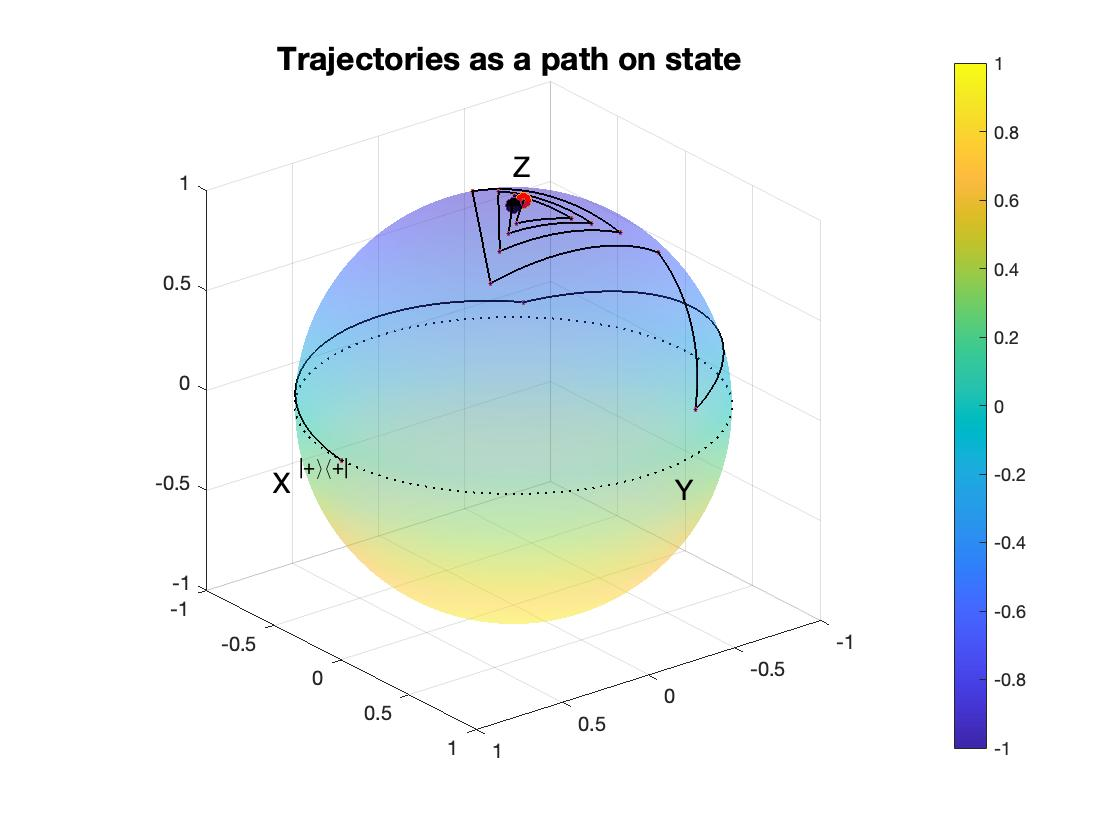
\includegraphics[width=0.5\textwidth]{images/1qubit_s.jpg} \label{ex1_e}}
        \subfloat[Mixed State Trajectory]{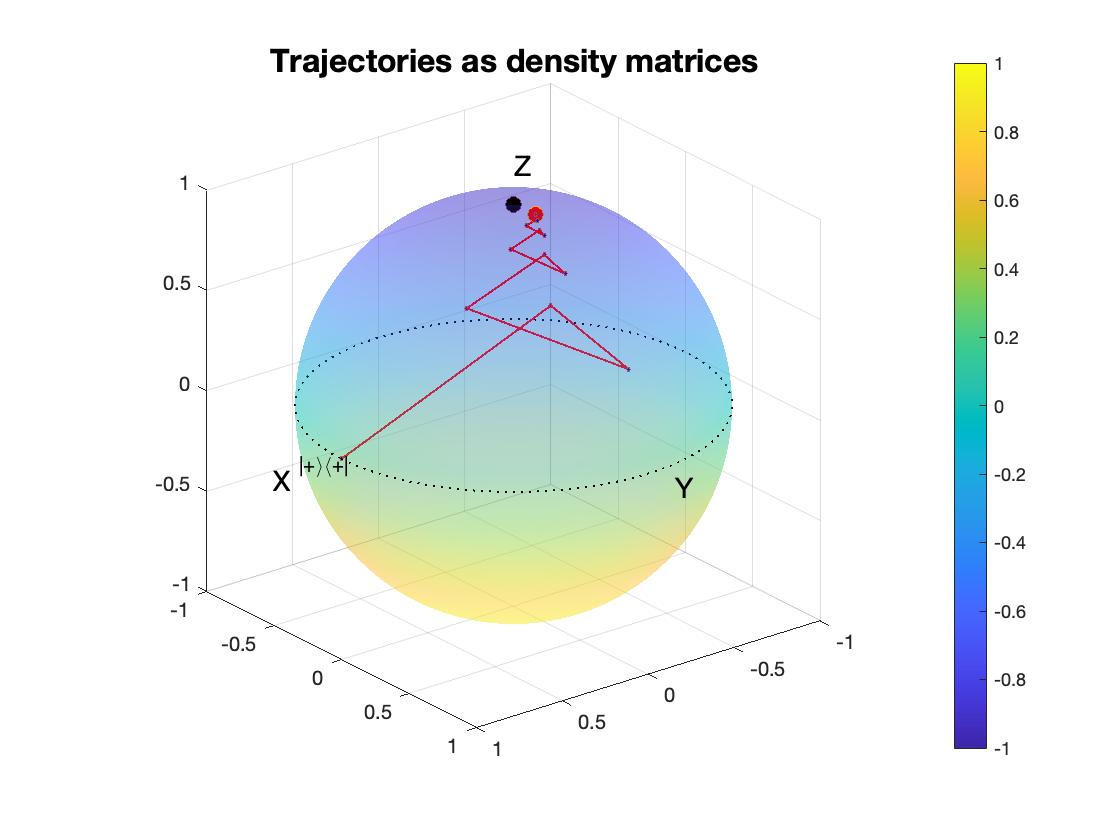
\includegraphics[width=0.5\textwidth]{images/1qubit_m.jpg} \label{ex1_e}}
        
    \caption{Example of the evolution of state with a single qubit -- see monotonicity!}
    \label{fig:enter-label}
\end{figure}

\subsection{General case}
Generically, for arbitrary Hamiltonians, 

\begin{figure}[h]
    \centering
        \subfloat[eigenvalues]{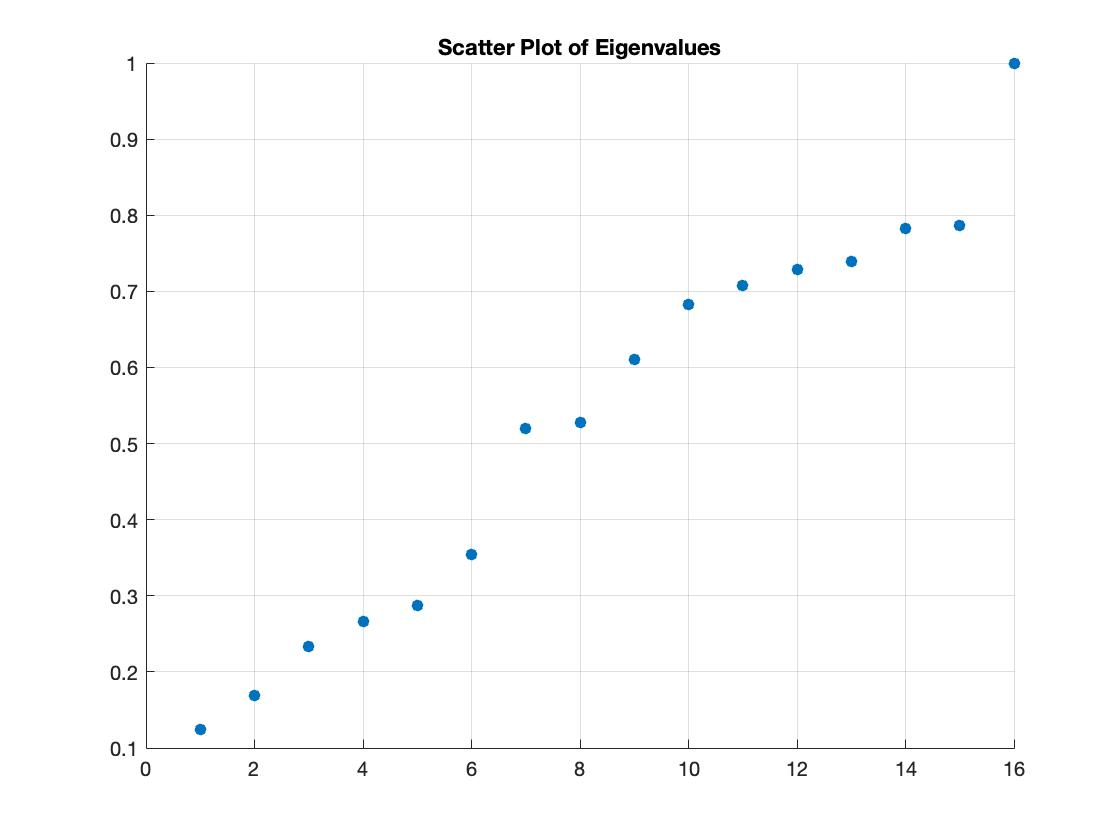
\includegraphics[width=0.3\textwidth]{images/ex1_eigvals.jpg} \label{ex1_e}}
        \subfloat[Initially lowest eigenstate]{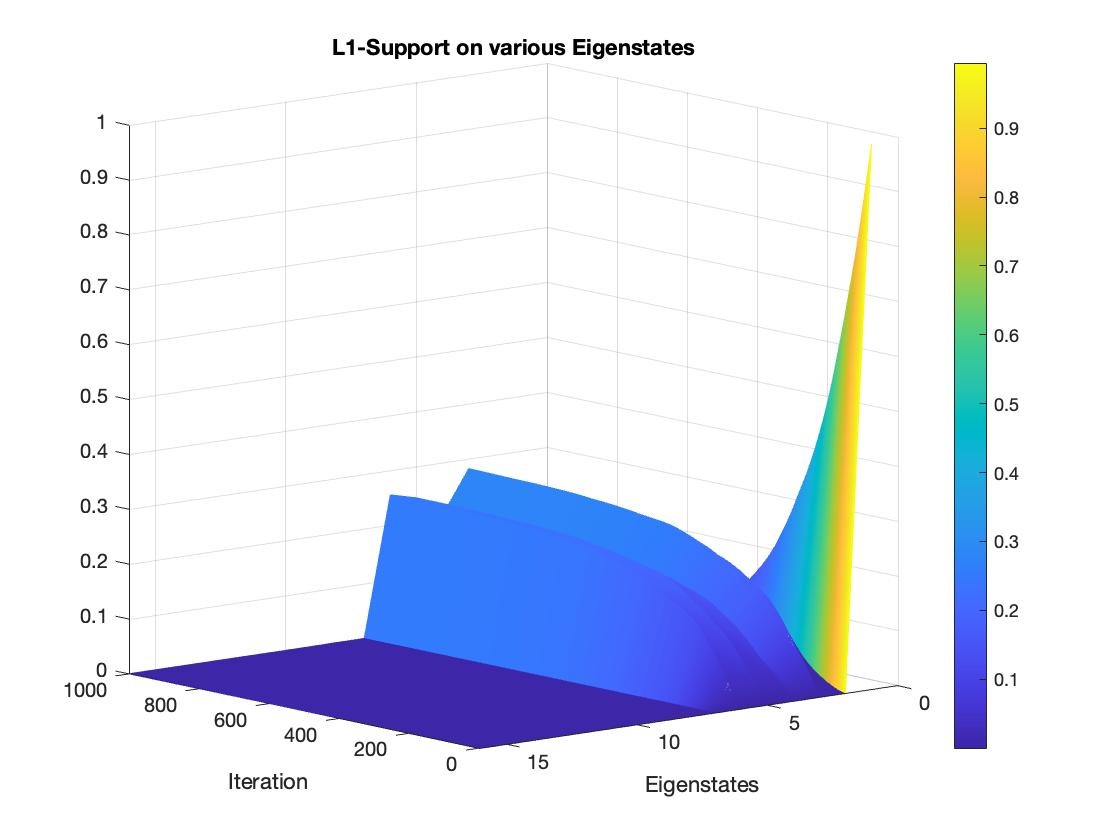
\includegraphics[width=0.3\textwidth]{images/ex1_eig1.jpg}\label{ex1_e1}}
        \subfloat[Initially mixed State]{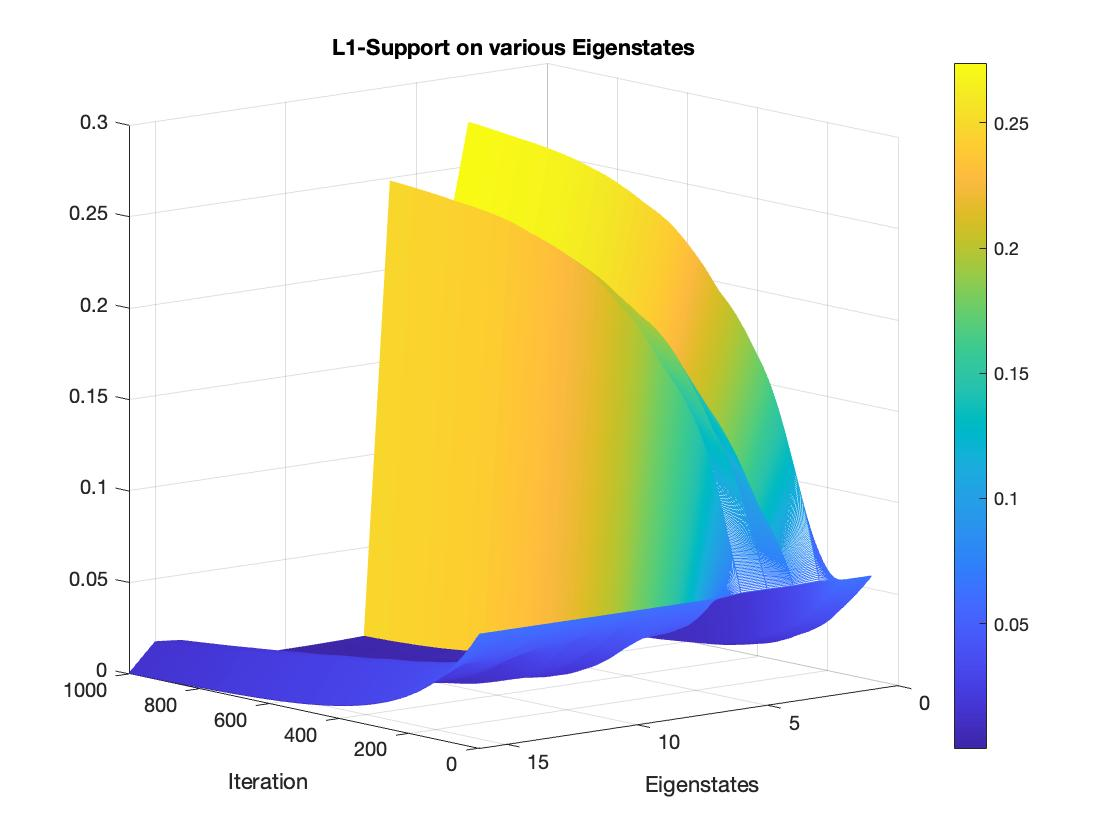
\includegraphics[width=0.3\textwidth]{images/ex1_mixed.jpg}\label{ex1_m}}
\\ 
        \subfloat[eigenvalues]{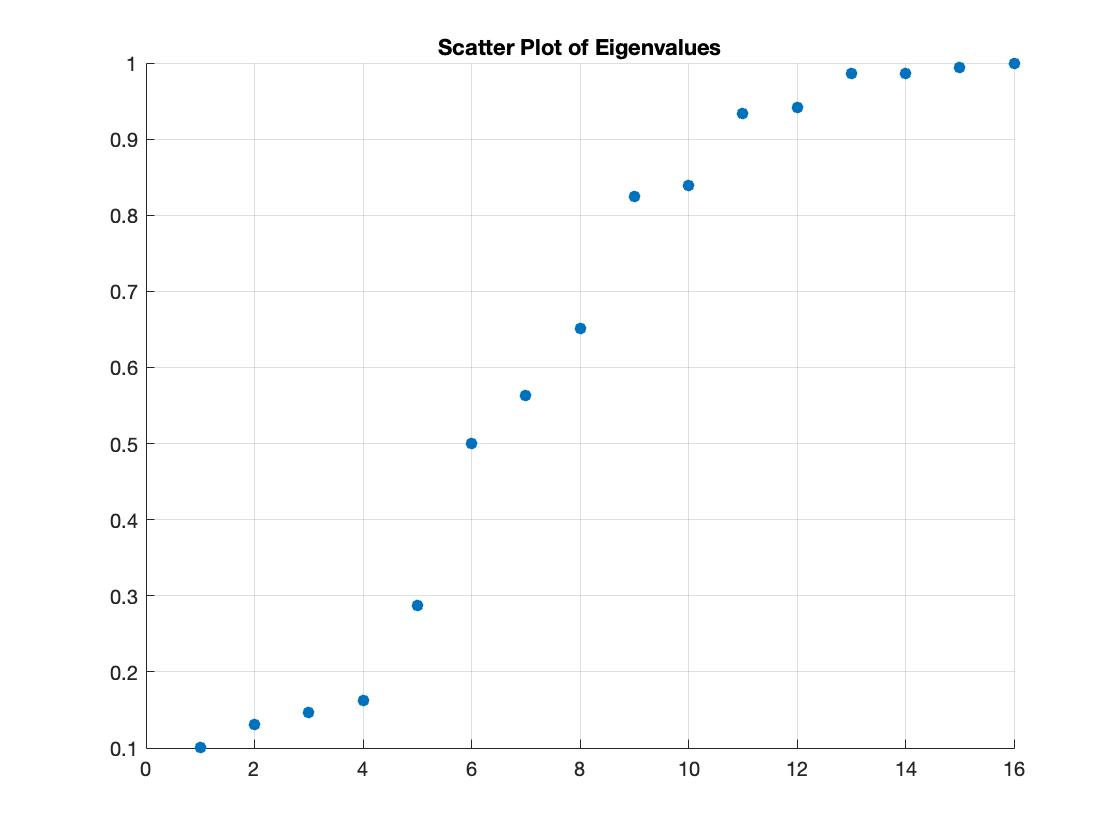
\includegraphics[width=0.3\textwidth]{images/ex2_eigvals.jpg} \label{ex2_e}}
        \subfloat[Initially lowest eigenstate]{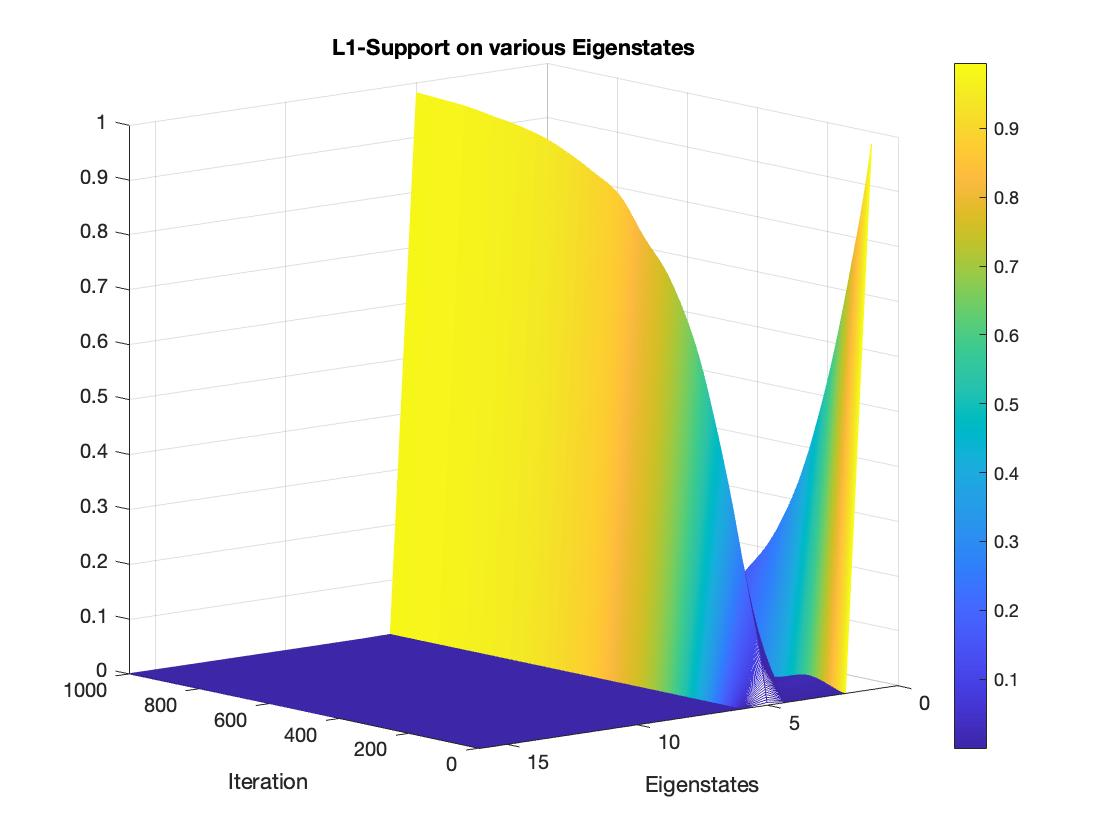
\includegraphics[width=0.3\textwidth]{images/ex2_eig1.jpg}\label{ex1_e1}}
        \subfloat[Initially mixed State]{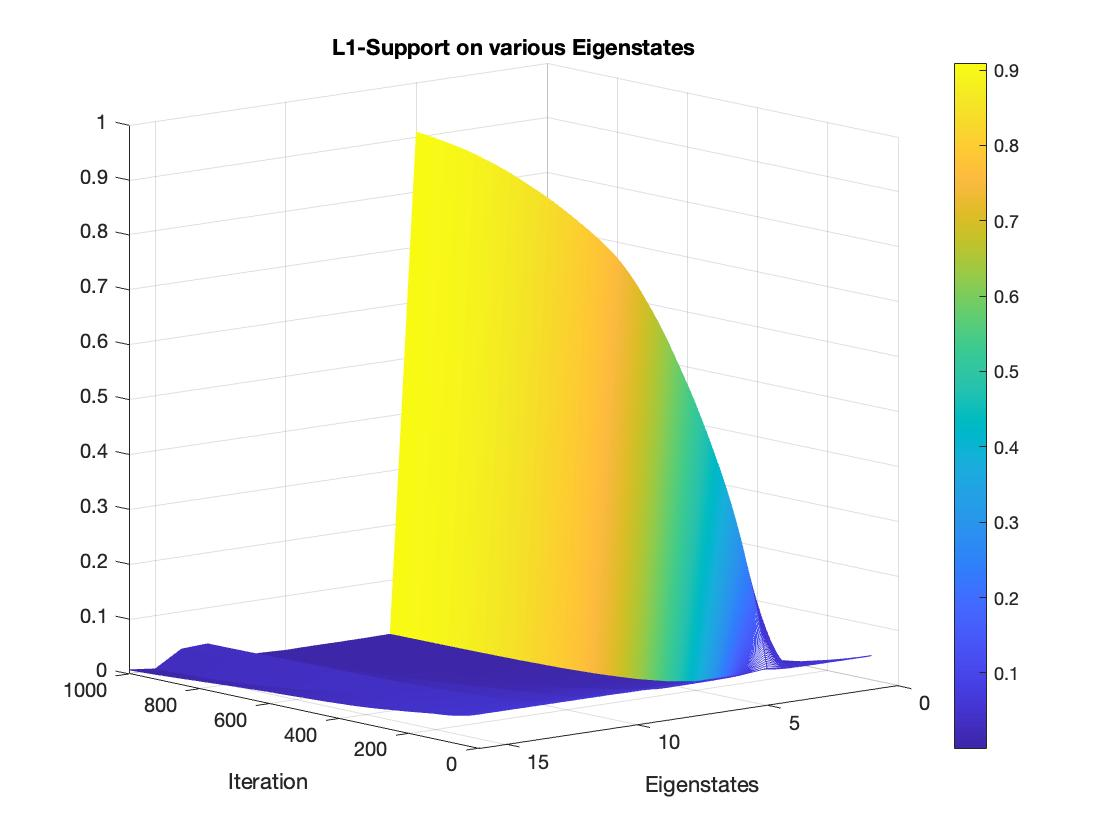
\includegraphics[width=0.3\textwidth]{images/ex2_mixed.jpg}\label{ex1_m}}
    \caption{Four Qubit examples with two different Hamiltonians. The left panel shows the eigenvalue distribution, the middle panel is when the initial state is the an eigenstate, the right panel is when the initial state is the maximally mixed state. See in each the weight from the states monotonically move the weights on the desired subspace}
\end{figure}

\subsection{Notes on scaling}

\textbf{Expt 1} (m=1 qubits): 
Counting minimum number of collisions to get $>0.8$ overlap, with, L0=0; L1=n; Hs = Diag(-N/2:N/2-1) \\
Run 1: $||Hs|| = n^2$; time=$1$, L= $1000n$; T=$50n$; \\
Run 2: $||Hs|| = n^2$; time=$n$, L= $2000\sqrt{n}$; T=$50\sqrt{n}$; \\
Run 3: $||Hs|| = n^2$; time=$\pi$, L= $2000\sqrt{n}$; T=$50\sqrt{n}$; \\
Run 4: $||Hs|| = n^2$; time=$1$, L= $2000$; T=$50$; (n=2:10, 20+14+50+374 mins runtime) \\

\noindent
n=2, 02 Collisions;  $\quad$  02 collisions, \quad  03 cols, \quad 03 cols \\
n=3, 22 Collisions, $\quad$ 19 collisions, \quad $16$ cols, \quad 15 cols  \\
n=4, 30 Collisions, $\quad$ 29 collisions, \quad $23$ cols, \quad 38 cols  \\
n=5, 31 Collisions, $\quad$ 33 collisions, \quad $46$ cols, \quad 34 cols  \\
n=6, 48 Collisions, \hspace{12em} \ 49 cols \\
n=7, 55 Collisions, \hspace{12em} \ 58 cols \\
n=8, 00 Collisions, \hspace{12em} \ 77 cols \\
n=9, 00 Collisions, \hspace{12em} \ 81 cols \\
n=10, 0 Collisions, \hspace{12em} \ 87 cols \\

\textbf{Expt 2} (m=$\lceil$ log(n) $\rceil$ qubits): 
Counting minimum number of collisions to get $>0.8$ overlap, with, \\ 
L0=0; L1=n; Hs = Diag(-N/2:N/2-1) \\
Run 1: $||Hs|| = n^2$; time=$1$, L= $2500$; T=$50$; (n=2:5) \\

\noindent
n=2 (2 eigstates) \quad  Collisions \\
n=3 (2 eigstates) \quad  Collisions \\
n=4 (3 eigstates) \quad  Collisions \\
n=5 (4 eigstates) \quad  Collisions \\
n=6 


\textbf{Expt 3} (m=n qubits): 
Counting minimum number of collisions to get $>0.8$ overlap, with, \\ 
L0=0; L1=n; Hs = Diag(-N/2:N/2-1) \\
Run 1: $||Hs|| = n^2$; time=$1$, L= $2500$; T=$50$; (n=2:5) \\

\noindent
n=2 (2 eigstates) \quad 03 Collisions \\
n=3 (2 eigstates) \quad 13 Collisions \\
n=4 (3 eigstates) \quad 22 Collisions \\
n=5 (4 eigstates) \quad 23 Collisions \\
n=6 

\textbf{Expts} (m=2 qubits)
L0 = -1/n; L1 = n; time = $\frac{\pi}{2}$ (decreasing as 0.999*time in each iteration), L=5000, T=50 (the large parameters are really to account for n=10 qubit run)

\begin{figure}[h]
    \centering
        \subfloat[Diagonal]{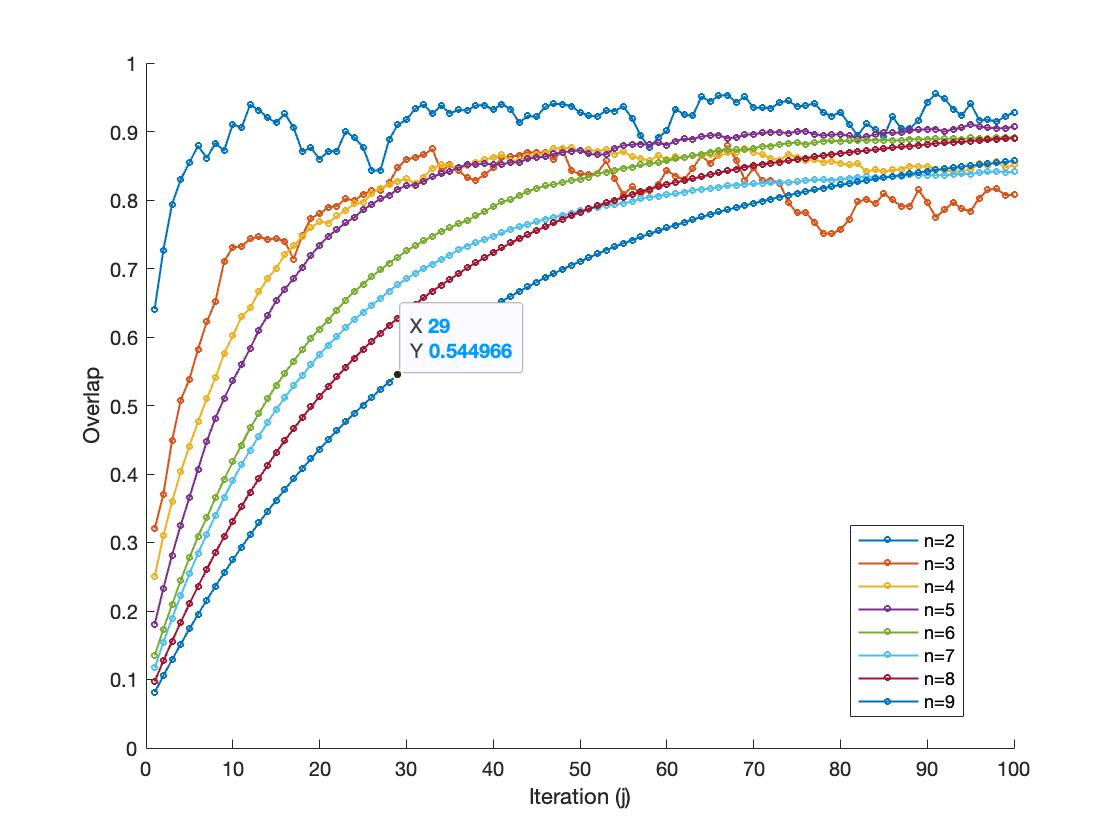
\includegraphics[width=0.5\textwidth]{images/Diagonal_1.jpg} \label{ex1_e}}
        \subfloat[XY Model]{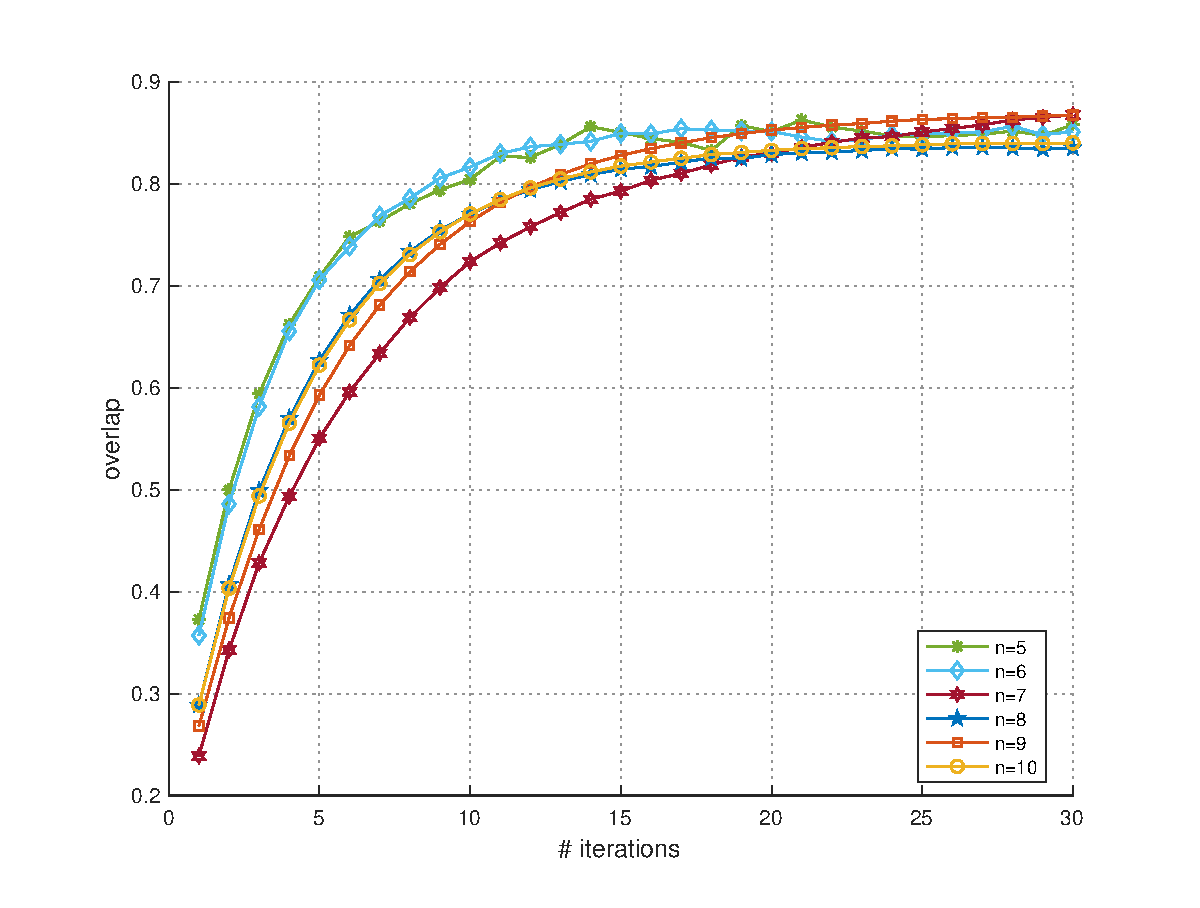
\includegraphics[width=0.5\textwidth]{images/xy_runs.eps}} \label{ex1_e}} \\
                \subfloat[Rate of convergence]{\includegraphics[width=0.5\textwidth]{images/rate_of_convergenc.jpg}} \label{ex2_e}

    \caption{Scaling in Diagonal}
\end{figure}




\end{document}



